\documentclass[12pt,a4paper,openany]{book}

% ========================
% PACKAGES
% ========================
\usepackage[utf8]{inputenc}
\usepackage[T1]{fontenc}
\usepackage[indonesian]{babel}
\usepackage{geometry}
\geometry{a4paper, left=3cm, right=2.5cm, top=2.5cm, bottom=2.5cm}
\usepackage{graphicx}
\usepackage{amsmath,amssymb,amsthm}
\theoremstyle{definition}
\newtheorem{example}{Contoh}
\usepackage{array}
\usepackage{enumitem}
\usepackage{xcolor}
\usepackage{hyperref}
\hypersetup{
  colorlinks=true,
  linkcolor=black,
  urlcolor=blue,
  citecolor=black
}
\usepackage{titlesec}
\usepackage{caption}
\usepackage{fancyhdr}

% ========================
% FORMATTING
% ========================
\captionsetup{font=small, labelfont=bf, skip=6pt}
\setlength{\parindent}{0pt}
\setlength{\parskip}{6pt}
\renewcommand{\arraystretch}{1.3}

\titleformat{\chapter}[display]
  {\normalfont\Large\bfseries\centering}
  {\chaptertitlename\ \thechapter}{12pt}{\Large}
\titlespacing*{\chapter}{0pt}{0pt}{30pt}

\pagestyle{fancy}
\fancyhf{}
\fancyhead[L]{\small\leftmark}
\fancyhead[R]{\small\thepage}
\renewcommand{\headrulewidth}{0.4pt}

% ========================
% BIBLIOGRAPHY
% ========================
% \usepackage[style=apa,backend=biber]{biblatex}
% \addbibresource{references.bib}

% ========================
% CUSTOM COMMANDS
% ========================
\newcommand{\miskonsepsi}[1]{\textbf{\textit{Miskonsepsi: #1}}}

% ========================
% DOCUMENT
% ========================
\begin{document}

% ---------- TITLE PAGE ----------
\begin{titlepage}
\centering
\vspace*{3cm}
{\Huge\bfseries LIMIT FUNGSI ALJABAR\par}
\vspace{0.5cm}
{\Large Pemahaman Konsep, Miskonsepsi, Faktor, dan Solusi\par}
\vspace{2cm}
{\Large BUKU AJAR\par}
\vspace{3cm}
{\large Disusun oleh\par}
\vspace{0.3cm}
{\large Aziz Nur Hafidz\par}
{\large NIM: 230102501022\par}
\vfill
{\large Program Studi Matematika\par}
{\large Fakultas Matematika dan Ilmu Pengetahuan Alam\par}
{\large Universitas Negeri Makassar\par}
{\large 2026\par}
\end{titlepage}

% ---------- KATA PENGANTAR ----------
\frontmatter
\chapter*{Kata Pengantar}
\addcontentsline{toc}{chapter}{Kata Pengantar}

Puji syukur penulis panjatkan ke hadirat Tuhan Yang Maha Esa atas selesainya penyusunan buku ajar \textit{Limit Fungsi Aljabar: Pemahaman Konsep, Miskonsepsi, Faktor, dan Solusi} ini.

Limit merupakan fondasi penting dalam kalkulus yang menjadi prasyarat bagi materi turunan, integral, dan kontinuitas fungsi. Namun, sifatnya yang abstrak sering menimbulkan hambatan epistemologis bagi siswa. Buku ini disusun sebagai bahan ajar yang tidak hanya membahas konsep dasar, tetapi juga secara khusus mengulas miskonsepsi yang umum dialami siswa, faktor penyebabnya, serta solusi didaktik yang dapat diterapkan guru.

Pembahasan dimulai dari definisi intuitif limit, limit kiri dan kanan, hingga tiga pendekatan pembelajaran (numerik, grafis, dan aljabar). Bagian utama buku ini menganalisis hasil kerja siswa, mengidentifikasi pola miskonsepsi, dan merumuskan strategi pembelajaran yang lebih bermakna. Dengan demikian, pembaca tidak hanya mengetahui prosedur penyelesaian, tetapi juga memahami alasan di balik setiap langkahnya.

Penulis menyadari bahwa buku ini masih memiliki kekurangan. Oleh karena itu, kritik dan saran yang membangun sangat penulis harapkan.

\vspace{1cm}
\begin{flushright}
Makassar, November 2026\\
\vspace{0.5cm}
Aziz Nur Hafidz
\end{flushright}

% ---------- DAFTAR ISI ----------
\tableofcontents
\listoffigures
\listoftables

% ---------- MAIN MATTER ----------
\mainmatter

% =====================================================
% FORCE CHAPTER TO START AT 11
% =====================================================
\setcounter{chapter}{10} % Makes the next chapter "BAB 11"

% =====================================================
% BAB 11: PENDAHULUAN
% =====================================================
\chapter{Pendahuluan}

\textbf{Tujuan Pembelajaran.} Setelah mempelajari bab ini, pembaca diharapkan mampu:
\begin{enumerate}
  \item menjelaskan pengertian limit fungsi aljabar secara intuitif;
  \item membedakan limit kiri dan limit kanan;
  \item memahami pendekatan numerik, grafis, dan aljabar dalam limit;
  \item mengidentifikasi miskonsepsi yang sering terjadi pada materi limit beserta konsep yang benar;
  \item menjelaskan faktor penyebab miskonsepsi dan solusi didaktiknya.
\end{enumerate}

\section{Latar Belakang}

Limit merupakan salah satu konsep fundamental dalam kalkulus yang menjadi fondasi bagi materi turunan, integral, dan kontinuitas fungsi. Namun, sifatnya yang abstrak sering menimbulkan hambatan epistemologis bagi siswa. Penelitian Fatuha et al. (2026) menunjukkan bahwa 53,3\% siswa kelas XI MIPA mengalami miskonsepsi pada materi limit fungsi aljabar. Miskonsepsi ini tidak hanya bersifat kognitif, tetapi juga dipengaruhi oleh faktor eksternal seperti pembelajaran prosedural dan keterbatasan waktu.

Tonra et al. (2025) menambahkan bahwa hambatan belajar pada limit bersifat epistemologis, psikologis-ontogenik, instrumental-ontogenik, dan konseptual-ontogenik. Definisi formal limit merupakan hambatan belajar yang paling sering muncul. Oleh karena itu, diperlukan analisis didaktik yang tidak hanya menemukan kesalahan siswa, tetapi juga merumuskan solusi pembelajaran yang efektif.

\section{Rumusan Masalah}

Berdasarkan latar belakang di atas, rumusan masalah dalam buku ini adalah:
\begin{enumerate}
  \item Bagaimana konsep dasar limit fungsi aljabar diajarkan di SMA?
  \item Jenis miskonsepsi apa saja yang dialami siswa pada materi limit fungsi aljabar?
  \item Faktor-faktor apa yang menyebabkan terjadinya miskonsepsi tersebut?
  \item Solusi apa yang dapat diterapkan untuk mengatasi miskonsepsi tersebut?
\end{enumerate}

% =====================================================
% BAB 12: KONSEP DASAR LIMIT FUNGSI ALJABAR
% =====================================================
\chapter{Konsep Dasar Limit Fungsi Aljabar}

\section{Definisi Intuitif}

Limit adalah nilai yang \textbf{didekati} oleh suatu fungsi $f(x)$ ketika variabel $x$ mendekati nilai tertentu $a$. Notasi
\[
\lim_{x \to a} f(x) = L
\]
berarti bahwa nilai $f(x)$ dapat dibuat sedekat mungkin dengan $L$ dengan mengambil $x$ yang cukup dekat dengan $a$, tetapi $x \neq a$.

Nilai limit tidak harus sama dengan nilai fungsi di titik tersebut, yaitu $f(a)$. Bahkan, fungsi tidak perlu terdefinisi di titik $a$ agar limitnya ada. Sebagai contoh, fungsi $f(x) = \frac{x^2-4}{x-2}$ tidak terdefinisi di $x = 2$, tetapi limitnya di $x = 2$ tetap ada, yaitu 4.

\section{Limit Kiri dan Limit Kanan}

Limit kiri ($x \to a^-$) adalah nilai yang didekati saat $x$ mendekati $a$ dari arah kiri (nilai lebih kecil dari $a$). Limit kanan ($x \to a^+$) adalah nilai yang didekati saat $x$ mendekati $a$ dari arah kanan (nilai lebih besar dari $a$).

Sebuah limit $\lim_{x \to a} f(x)$ dikatakan ada jika dan hanya jika:
\[
\lim_{x \to a^-} f(x) = \lim_{x \to a^+} f(x) = L.
\]
Jika limit kiri dan limit kanan berbeda, maka limit di titik tersebut tidak ada.

\section{Pendekatan Pembelajaran Limit}

\subsection{Pendekatan Numerik (Tabel)}

Salah satu cara memahami limit adalah melalui pendekatan numerik, yaitu membuat tabel nilai fungsi untuk $x$ yang mendekati $a$ dari kiri dan kanan. Sebagai contoh, perhatikan limit berikut:
\[
\lim_{x \to 2} \frac{x^2 - 4}{x - 2}.
\]
Jika kita substitusi langsung $x = 2$, diperoleh bentuk tak tentu $\frac{0}{0}$. Namun, dengan pendekatan numerik kita dapat mengamati perilaku fungsi di sekitar $x = 2$.

\begin{table}[h]
\centering
\caption{Pendekatan Numerik $\lim_{x \to 2} \frac{x^2-4}{x-2}$}
\label{tab:numerik}
\begin{tabular}{@{}cccc@{}}
\toprule
\multicolumn{2}{c}{\textbf{Dari Kiri ($x < 2$)}} & \multicolumn{2}{c}{\textbf{Dari Kanan ($x > 2$)}} \\
\cmidrule(lr){1-2} \cmidrule(lr){3-4}
$x$ & $f(x)$ & $x$ & $f(x)$ \\
\midrule
1,9 & 3,9 & 2,1 & 4,1 \\
1,99 & 3,99 & 2,01 & 4,01 \\
1,999 & 3,999 & 2,001 & 4,001 \\
1,9999 & 3,9999 & 2,0001 & 4,0001 \\
\bottomrule
\end{tabular}
\end{table}

Dari Tabel \ref{tab:numerik} terlihat bahwa ketika $x$ mendekati 2 dari kiri maupun kanan, nilai $f(x)$ mendekati 4. Dengan demikian, $\lim_{x \to 2} \frac{x^2-4}{x-2} = 4$.

\subsection{Pendekatan Grafis}

Selain tabel, pendekatan grafis dapat memberikan gambaran visual tentang perilaku fungsi di sekitar titik yang didekati. Grafik fungsi $f(x) = \frac{x^2-4}{x-2}$ sebenarnya identik dengan garis $y = x + 2$, tetapi memiliki \textit{hole} (lubang) di $x = 2$ karena fungsi tidak terdefinisi di titik tersebut.

Saat $x$ mendekati 2, baik dari kiri maupun kanan, kurva mengarah ke nilai $y = 4$. Titik $(2, 4)$ sendiri tidak termasuk dalam grafik, tetapi limitnya tetap ada.

\subsection{Pendekatan Aljabar}

Pendekatan aljabar dilakukan dengan manipulasi bentuk fungsi, seperti faktorisasi, rasionalisasi, dan pembagian. Untuk contoh di atas:
\[
\lim_{x \to 2} \frac{x^2 - 4}{x - 2} = \lim_{x \to 2} \frac{(x - 2)(x + 2)}{x - 2} = \lim_{x \to 2} (x + 2) = 4.
\]
Pendekatan ini memberikan hasil yang eksak dan menjadi cara utama dalam menyelesaikan limit fungsi aljabar.

% =====================================================
% BAB 13: MISKONSEPSI PADA MATERI LIMIT FUNGSI ALJABAR
% =====================================================
\chapter{Miskonsepsi pada Materi Limit Fungsi Aljabar}

Berdasarkan penelitian Fatuha et al. (2026) dan analisis lembar jawaban siswa, ditemukan lima pola miskonsepsi utama pada materi limit fungsi aljabar.

\section{Miskonsepsi 1: Substitusi Langsung Tanpa Analisis}

\miskonsepsi{Siswa langsung memasukkan nilai $x$ ke dalam fungsi tanpa mengecek apakah hasilnya bentuk tak tentu.}

Berdasarkan data penelitian, miskonsepsi ini terjadi pada \textbf{93,8\%} siswa dalam kategori miskonsepsi (Fatuha et al., 2026). Siswa beranggapan bahwa semua limit dapat diselesaikan dengan substitusi langsung. 

Kutipan siswa (S2): \textit{``Saya selalu langsung masukkan angkanya, karena guru bilang cari nilai limit ya substitusi.''}

\begin{example}
Hitunglah $\displaystyle \lim_{x \to 1} \frac{x^2 - 1}{x - 1}$.

Siswa menjawab $\frac{0}{0}$ lalu berhenti. Padahal jawaban yang benar adalah 2, yang diperoleh melalui pemfaktoran.
\end{example}

\section{Miskonsepsi 2: Kesalahan Memahami Bentuk Tak Tentu $\frac{0}{0}$}

\miskonsepsi{Siswa menganggap $\frac{0}{0}$ sebagai hasil akhir (jawaban nol) atau sebagai tanda bahwa limit tidak ada.}

Miskonsepsi ini terjadi pada \textbf{87,5\%} siswa dalam kategori miskonsepsi (Fatuha et al., 2026). 

Kutipan siswa (S4): \textit{``Kalau dapat 0/0, saya pikir jawabannya nol atau tidak ada, karena dibagi nol kan tidak boleh.''}

Fakta pentingnya, $\frac{0}{0}$ adalah sinyal untuk melakukan manipulasi aljabar (faktorisasi/rasionalisasi), \textbf{bukan} jawaban akhir. Konsep yang benar:
\[
\lim_{x \to 2} \frac{x^2 - 4}{x - 2} = \lim_{x \to 2} \frac{(x - 2)(x + 2)}{x - 2} = \lim_{x \to 2} (x + 2) = 4.
\]

\section{Miskonsepsi 3: Kesalahan Operasi Aljabar Prasyarat}

\miskonsepsi{Siswa tidak mampu memfaktorkan, menyederhanakan pecahan, atau merasionalkan bentuk akar dengan benar dalam konteks limit.}

Miskonsepsi ini terjadi pada \textbf{81,3\%} siswa dalam kategori miskonsepsi (Fatuha et al., 2026).

Kutipan siswa (S1): \textit{``Saya hafal $(a + b)(a - b)$, tapi kalau bentuknya $x^2 - 4$ saya bingung mau diubah jadi apa.''}

Contoh kesalahan:
\[
x^2 - 4 \neq (x - 2)(x - 2) \quad (\text{Salah})
\]
\[
x^2 - 4 = (x - 2)(x + 2) \quad (\text{Benar})
\]

\section{Miskonsepsi 4: Limit Sebagai Nilai Akhir (Bukan Proses)}

\miskonsepsi{Siswa menganggap limit sama persis dengan nilai fungsi di titik tersebut ($\lim_{x \to a} f(x) = f(a)$).}

Miskonsepsi ini terjadi pada \textbf{75,0\%} siswa dalam kategori miskonsepsi (Fatuha et al., 2026).

Kutipan siswa (S5): \textit{``Limit ya nilai di titik itu, sama saja kayak fungsi biasa.''}

Implikasinya, siswa gagal memahami bahwa limit mendeskripsikan perilaku mendekati, bukan nilai tepat di titik (terutama pada fungsi yang memiliki lubang/\textit{hole}).

\section{Miskonsepsi 5: Definisi Formal $\varepsilon$-$\delta$ Direduksi Menjadi Prosedur}

\miskonsepsi{Siswa menghafal langkah pembuktian $\varepsilon$-$\delta$ tanpa memahami maknanya.}

Berdasarkan analisis lembar jawaban, siswa dapat menuliskan langkah-langkah formal, tetapi tidak memahami bahwa $\varepsilon$ diberikan dan $\delta$ harus ditentukan. Akibatnya, ketika soal divariasikan, siswa tidak dapat menyelesaikannya. Miskonsepsi ini sejalan dengan temuan Tonra et al. (2025) yang menyatakan bahwa definisi formal limit merupakan hambatan belajar yang paling sering muncul.

\section{Dominasi Miskonsepsi}

\begin{table}[h]
\centering
\caption{Dominasi Miskonsepsi pada Materi Limit Fungsi Aljabar}
\label{tab:dominasi}
\begin{tabular}{@{}clc@{}}
\toprule
\textbf{No} & \textbf{Jenis Miskonsepsi} & \textbf{Persentase} \\
\midrule
1 & Substitusi langsung tanpa analisis & 93,8\% \\
2 & Kesalahan bentuk tak tentu $\frac{0}{0}$ & 87,5\% \\
3 & Kesalahan aljabar prasyarat & 81,3\% \\
4 & Limit sebagai nilai akhir & 75,0\% \\
\bottomrule
\end{tabular}
\end{table}

Dominasi miskonsepsi pada Tabel \ref{tab:dominasi} menunjukkan bahwa pemahaman siswa bersifat \textbf{instrumental} (prosedural), bukan \textbf{relasional} (konseptual). Data ini berdasarkan studi kasus pada 30 siswa di satu Madrasah Aliyah (Fatuha et al., 2026).

% =====================================================
% BAB 14: ANALISIS HASIL KERJA SISWA
% =====================================================
\chapter{Analisis Hasil Kerja Siswa}

Untuk melihat manifestasi nyata dari miskonsepsi di atas, dilakukan analisis terhadap tiga lembar jawaban siswa: satu jawaban lengkap (Putri) dan dua jawaban tidak lengkap (Nur Annisa dan satu siswa tanpa nama). 

\section{Instrumen Diagnostik (Soal)}
Berikut adalah soal yang diberikan kepada siswa. Petunjuk pengerjaan menekankan agar siswa menuliskan langkah pengerjaan, alasan pemilihan prosedur, dan penjelasan jika muncul bentuk tak tentu.

\begin{enumerate}[label=\textbf{\arabic*.}]
    \item Hitunglah kedua limit berikut.
    \[
    \text{(a) } \lim_{x\to 2}(3x+1)
    \qquad\qquad
    \text{(b) } \lim_{x\to 2}\frac{x^2-4}{x-2}
    \]
    Untuk masing-masing soal, tuliskan dahulu hasil substitusi langsung \(x=2\). Kemudian jelaskan mengapa cara yang berhasil pada (a) belum cukup untuk menyelesaikan (b).

    \item Hitunglah \(\displaystyle \lim_{x\to 3}\frac{x^2-9}{x-3}\). Tuliskan seluruh langkah pengerjaanmu, termasuk hasil substitusi langsung dan penjelasan tentang hasil tersebut.

    \item Sederhanakan bentuk \(\dfrac{\sqrt{x}-2}{x-4}\) untuk \(x\ne 4\), kemudian tentukan \(\displaystyle \lim_{x\to 4}\frac{\sqrt{x}-2}{x-4}\).

    \item Diketahui \(f(x)=\dfrac{x^2-1}{x-1}\quad (x\ne 1)\), dan \(f(1)=4\). Tentukan \(\displaystyle \lim_{x\to 1} f(x)\) dan \(f(1)\). Apakah kedua nilai itu sama? Jelaskan.

    \item Diberikan \(\displaystyle \lim_{x\to 2}(3x+1)=7\).
    \begin{enumerate}[label=(\alph*)]
        \item Tuliskan \(|(3x+1)-7|\) dalam bentuk \(k\,|x-2|\).
        \item Dengan definisi \(\varepsilon-\delta\), tentukan suatu \(\delta>0\) dalam bentuk \(\varepsilon\) sehingga \(0<|x-2|<\delta \implies |(3x+1)-7|<\varepsilon\).
    \end{enumerate}
\end{enumerate}

\section{Jawaban Lengkap (Putri)}

Siswa atas nama Putri mengerjakan seluruh soal dengan tuntas dan memberikan justifikasi tertulis yang sangat baik di setiap langkahnya. Putri menuliskan bahwa substitusi langsung pada soal nomor 1b menghasilkan bentuk tak tentu, sehingga ia melanjutkan dengan pemfaktoran. Pada soal nomor 3, Putri melakukan perasionalan dengan benar. Pada soal nomor 5, Putri menyelesaikan pembuktian $\varepsilon$-$\delta$ dengan menentukan $\delta = \varepsilon/3$.

Jawaban Putri dapat dilihat pada Gambar \ref{fig:putri1} dan Gambar \ref{fig:putri2}.

\begin{figure}[h]
\centering
% 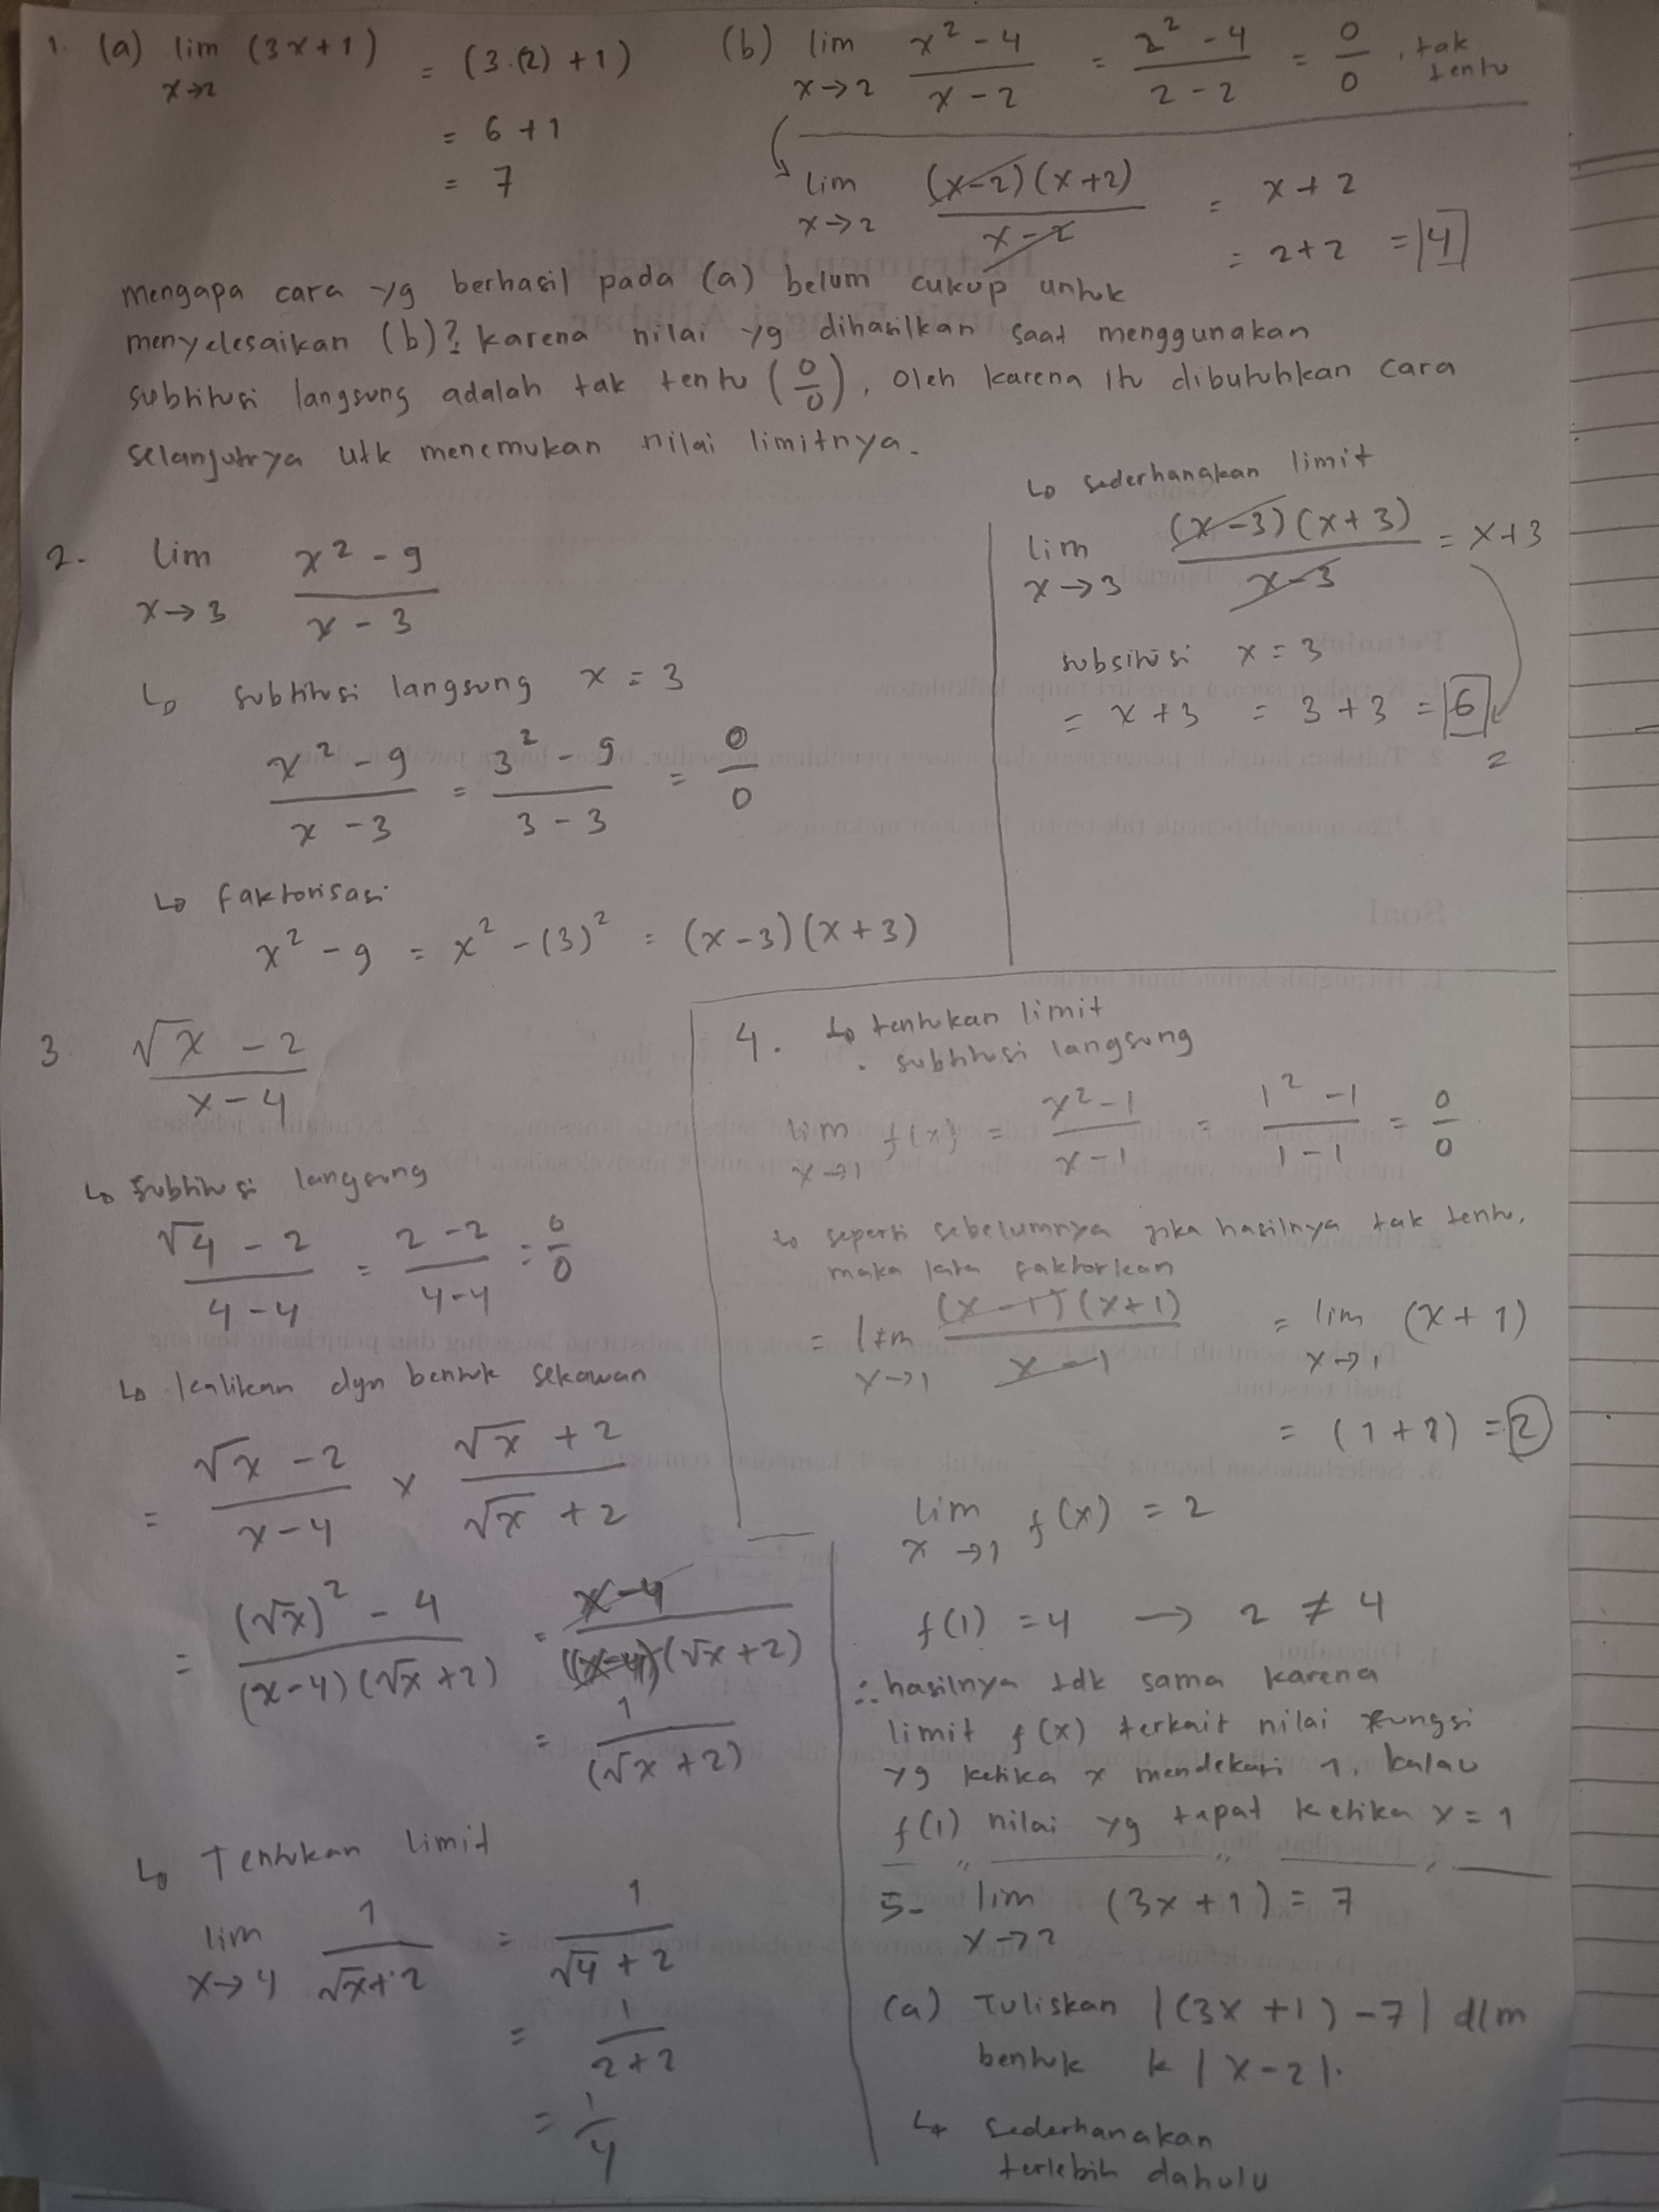
\includegraphics[width=0.7\textwidth]{gambar1.jpg}
\fbox{\parbox[c][6cm][c]{0.7\textwidth}{\centering\itshape Gambar tidak tersedia}}
\caption{Halaman 1 Jawaban Putri}
\label{fig:putri1}
\end{figure}

\begin{figure}[h]
\centering
% 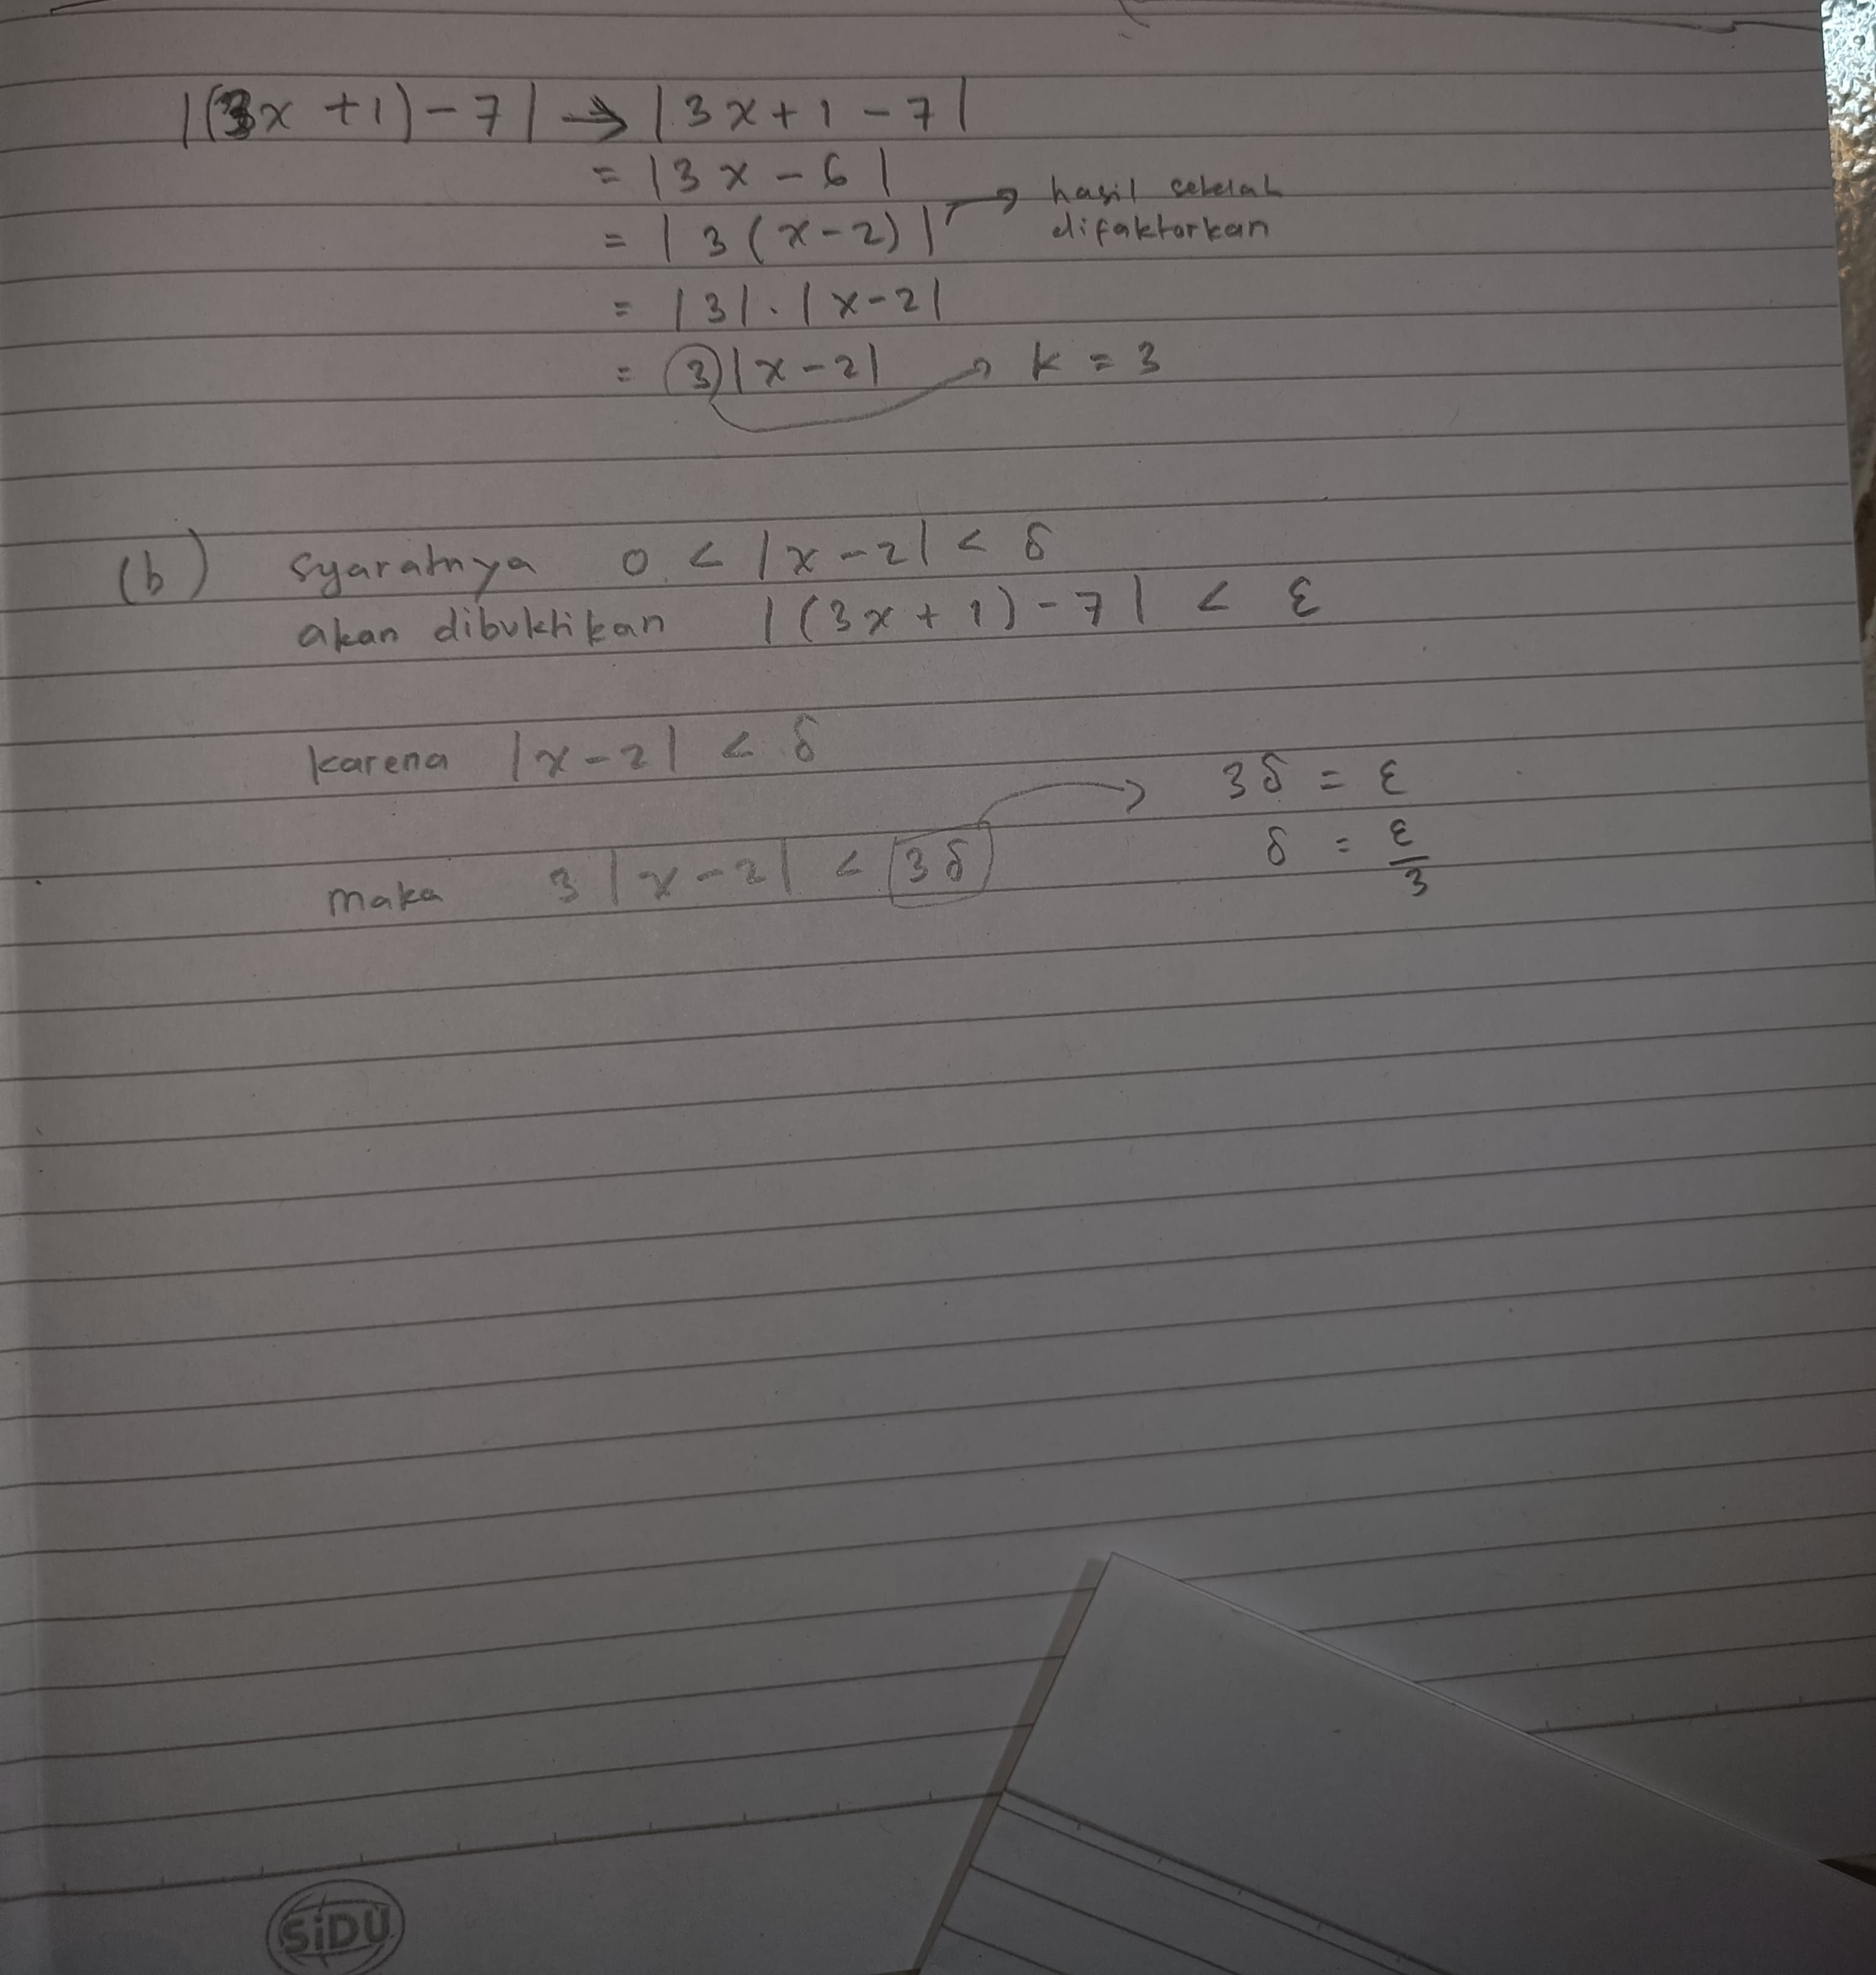
\includegraphics[width=0.7\textwidth]{gambar2.jpg}
\fbox{\parbox[c][6cm][c]{0.7\textwidth}{\centering\itshape Gambar tidak tersedia}}
\caption{Halaman 2 Jawaban Putri}
\label{fig:putri2}
\end{figure}

\section{Jawaban Tidak Lengkap (Nur Annisa dan Tanpa Nama)}

Berbeda dengan Putri, Nur Annisa dan satu siswa tanpa nama tidak menyelesaikan soal nomor 3, 4, dan 5 secara tuntas. Ketidaklengkapan ini bukan sekadar karena keterbatasan waktu, melainkan indikasi kuat adanya miskonsepsi dan kegagalan manipulasi aljabar.

Pada soal nomor 4, Nur Annisa melakukan substitusi langsung dan menuliskan hasil $\frac{1^2 - 1}{1 - 1} = \frac{0}{0}$, lalu berhenti di titik tersebut. Ia menganggap $\frac{0}{0}$ sebagai hasil akhir yang sah, bukan sebagai sinyal untuk melakukan faktorisasi. Akibatnya, ia tidak dapat membandingkan bahwa $\lim_{x \to 1} f(x) = 2$ berbeda dengan $f(1) = 4$.

Pada soal nomor 3, salah satu siswa berhenti pada tahap substitusi $\frac{4^{1/2} - 2}{4 - 4} = \frac{0}{0}$ dan tidak melanjutkan pengerjaan, sementara siswa lainnya membiarkannya kosong. Hal ini menunjukkan bahwa siswa tidak menguasai teknik perkalian sekawan untuk menghilangkan bentuk akar pada pembilang.

Pada soal nomor 5, lembar jawaban untuk pembuktian limit dengan definisi formal $\varepsilon$-$\delta$ dibiarkan kosong. Ini mengindikasikan bahwa definisi formal direduksi menjadi prosedur, atau bahkan sama sekali tidak dipahami karena dianggap terlalu abstrak.

Jawaban tidak lengkap dapat dilihat pada Gambar \ref{fig:tidaklengkap1} dan Gambar \ref{fig:tidaklengkap2}.

\begin{figure}[h]
\centering
% 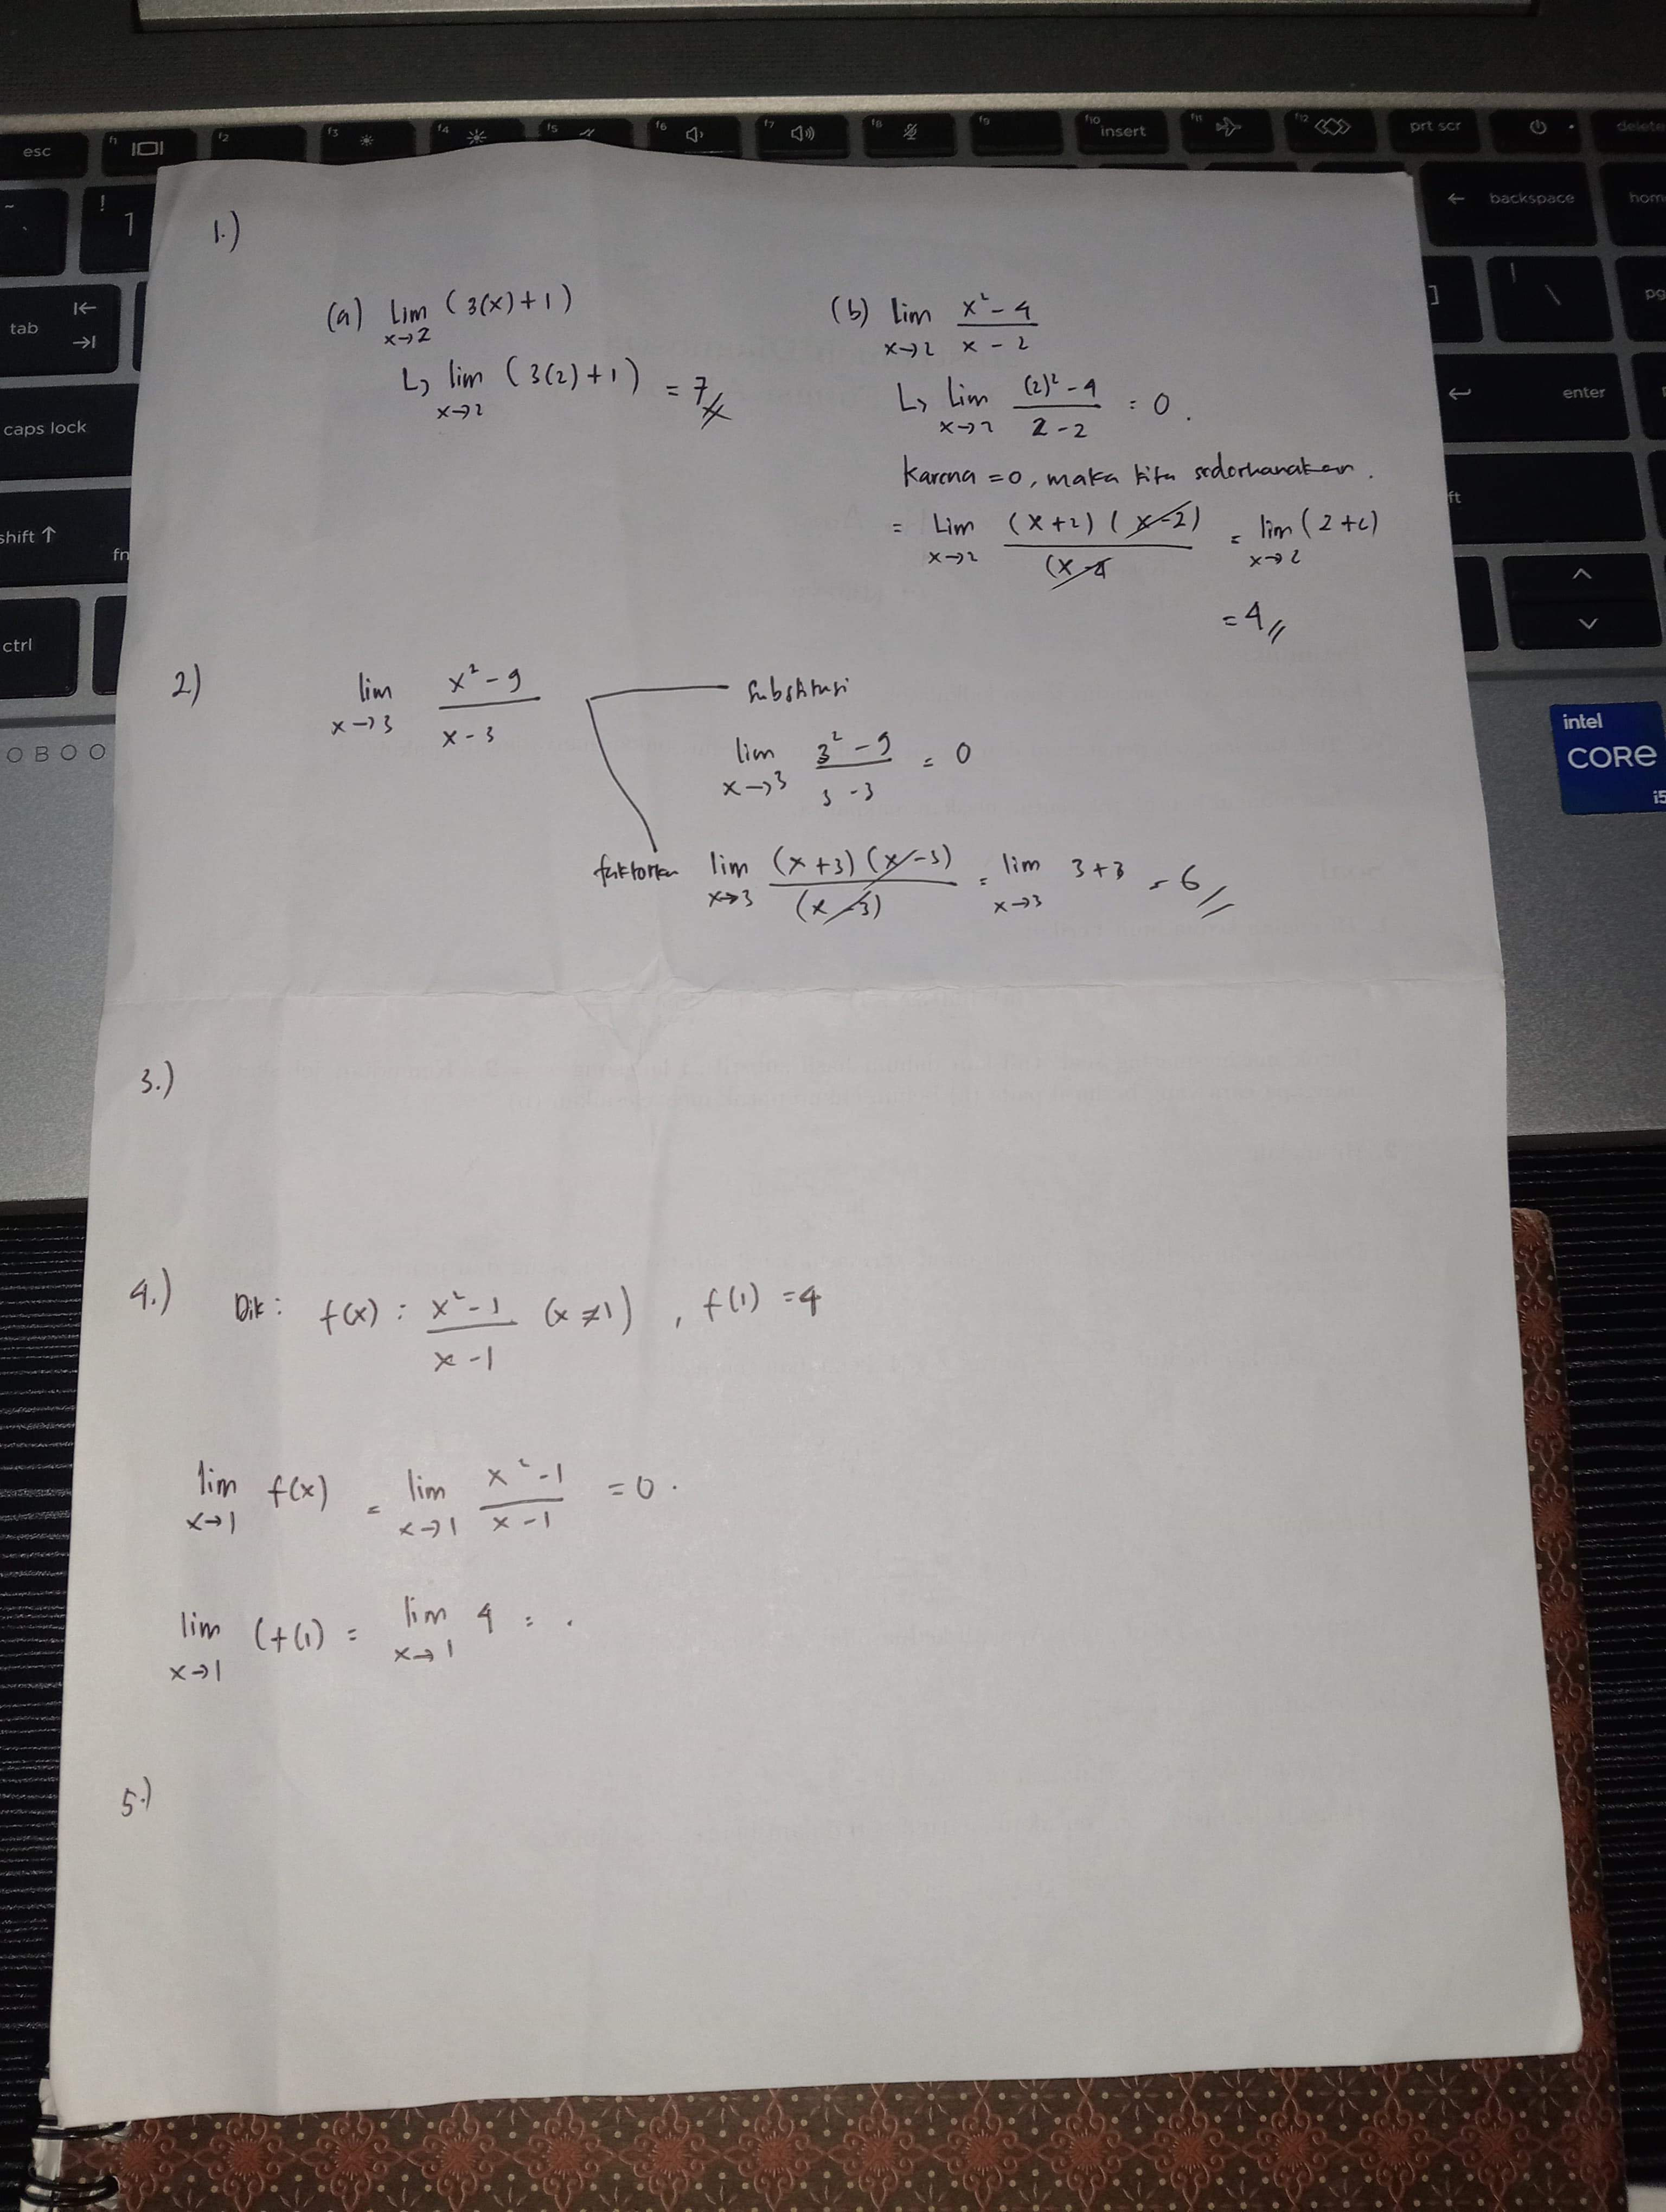
\includegraphics[width=0.7\textwidth]{gambar3.jpg}
\fbox{\parbox[c][6cm][c]{0.7\textwidth}{\centering\itshape Gambar tidak tersedia}}
\caption{Jawaban Tidak Lengkap (Tanpa Nama)}
\label{fig:tidaklengkap1}
\end{figure}

\begin{figure}[h]
\centering
% 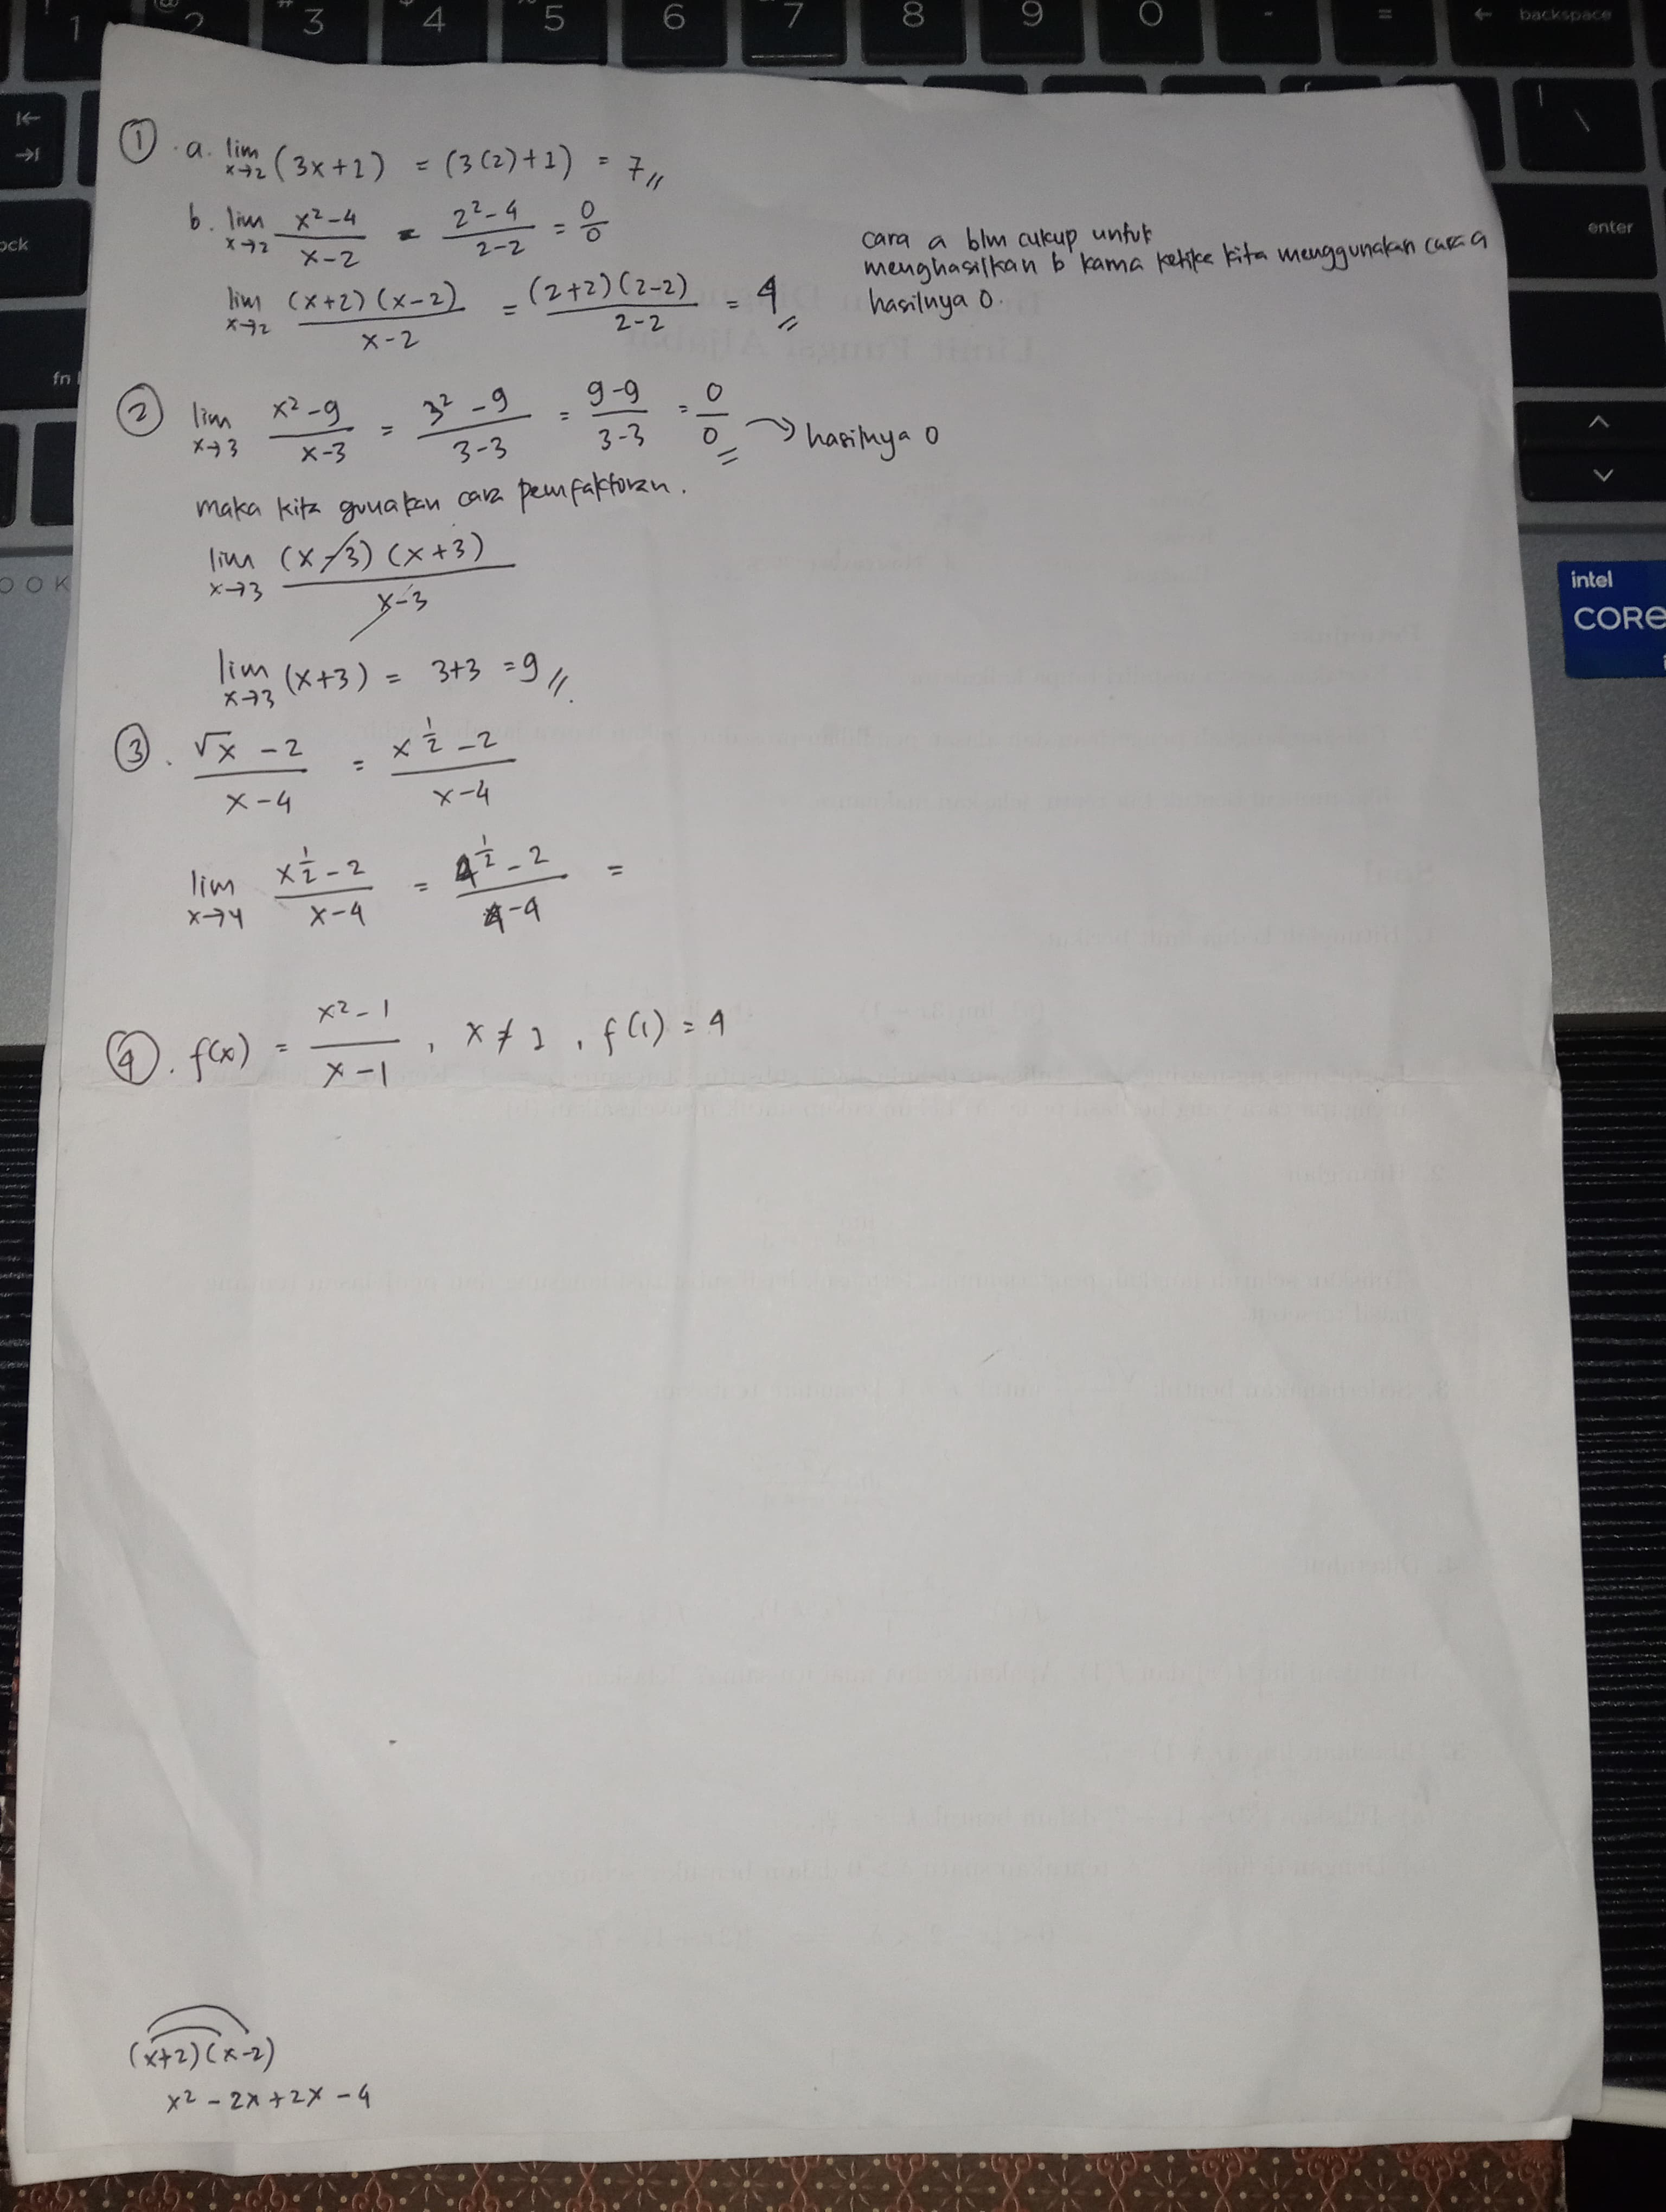
\includegraphics[width=0.7\textwidth]{gambar4.jpg}
\fbox{\parbox[c][6cm][c]{0.7\textwidth}{\centering\itshape Gambar tidak tersedia}}
\caption{Jawaban Tidak Lengkap (Nur Annisa)}
\label{fig:tidaklengkap2}
\end{figure}

\section{Kunci Jawaban Instrumen Diagnostik}

Sebagai pembanding, berikut adalah kunci jawaban dari instrumen diagnostik yang diberikan.

\begin{enumerate}[label=\textbf{\arabic*.}]
    \item 
    \begin{enumerate}[label=(\alph*)]
        \item Substitusi langsung: \(3(2)+1=7\). Jadi \(\displaystyle \lim_{x\to2}(3x+1)=7\).
        \item Substitusi langsung: \(\dfrac{2^2-4}{2-2}=\dfrac{0}{0}\) (bentuk tak tentu). Faktorkan: \(\frac{x^2-4}{x-2}=\frac{(x-2)(x+2)}{x-2}=x+2\), sehingga limitnya \(2+2=4\).
    \end{enumerate}
    Pada (a) fungsi kontinu di \(x=2\), sehingga substitusi langsung sah. Pada (b) substitusi langsung menghasilkan bentuk tak tentu, sehingga masih diperlukan manipulasi aljabar.

    \item Substitusi langsung: \(\frac{3^2-9}{3-3}=\frac{0}{0}\). Faktorkan: \(\frac{x^2-9}{x-3}=\frac{(x-3)(x+3)}{x-3}=x+3\), sehingga \(\lim_{x\to3}\frac{x^2-9}{x-3}=3+3=6\).

    \item Kalikan dengan sekawan: \(\frac{\sqrt{x}-2}{x-4}=\frac{(\sqrt{x}-2)(\sqrt{x}+2)}{(x-4)(\sqrt{x}+2)}=\frac{x-4}{(x-4)(\sqrt{x}+2)}=\frac{1}{\sqrt{x}+2}\). Jadi, \(\lim_{x\to4}\frac{\sqrt{x}-2}{x-4}=\frac{1}{\sqrt{4}+2}=\frac{1}{4}\).

    \item \(\lim_{x\to1}\frac{x^2-1}{x-1}=\lim_{x\to1}\frac{(x-1)(x+1)}{x-1}=\lim_{x\to1}(x+1)=2\), sedangkan \(f(1)=4\). Jadi limit dan nilai fungsi tidak sama; limit mendeskripsikan nilai yang didekati \(f(x)\) saat \(x\) mendekati \(1\), bukan nilai fungsi tepat di \(x=1\).

    \item 
    \begin{enumerate}[label=(\alph*)]
        \item \(|(3x+1)-7|=|3x-6|=3|x-2|\).
        \item Karena \(3|x-2|<\varepsilon\) setara dengan \(|x-2|<\dfrac{\varepsilon}{3}\), maka dapat dipilih \(\delta=\frac{\varepsilon}{3}\).
    \end{enumerate}
\end{enumerate}

\section{Konfirmasi Teori}

Ketidaklengkapan jawaban di atas relevan dengan data penelitian Fatuha et al. (2026) yang menyatakan bahwa tingkat dominasi miskonsepsi pada siswa sangat tinggi. Meskipun siswa berhasil mengerjakan soal nomor 1 dan 2 (menemukan nilai limit 4 dan 6 melalui faktorisasi), keberhasilan ini bersifat \textit{instrumental} (hafalan prosedur). Begitu dihadapkan pada variasi soal yang lebih kompleks---seperti bentuk akar, perbandingan nilai fungsi, dan definisi formal $\varepsilon$-$\delta$---pemahaman \textit{relasional} siswa runtuh.

% =====================================================
% BAB 15: FAKTOR PENYEBAB MISKONSEPSI
% =====================================================
\chapter{Faktor Penyebab Miskonsepsi}

\section{Faktor Internal}

\begin{enumerate}
  \item \textbf{Penguasaan Prasyarat Lemah}: Siswa tidak menguasai materi aljabar dasar (faktorisasi, operasi pecahan, rasionalisasi) dengan baik.
  \item \textbf{Kebiasaan Menghafal Tanpa Memahami}: Siswa menghafal rumus-rumus aljabar tanpa memahami kapan dan mengapa prosedur tersebut digunakan dalam konteks limit.
  \item \textbf{Kurangnya Kesadaran Metakognitif}: Siswa tidak terbiasa mengecek kembali langkah-langkah pengerjaan atau bertanya apakah prosedur yang digunakan sudah tepat.
\end{enumerate}

\section{Faktor Eksternal}

\begin{enumerate}
  \item \textbf{Pembelajaran Prosedural}: Guru mengajarkan ``langkah-langkah'' tanpa menjelaskan makna di baliknya (misal: langsung mengajarkan faktorisasi tanpa menunjukkan grafik/tabel).
  \item \textbf{Keterbatasan Waktu}: Kurikulum yang padat menyebabkan guru terburu-buru menyelesaikan materi, sehingga penguatan konsep kurang optimal.
  \item \textbf{Kontrak Didaktik Implisit}: Terbentuk keyakinan di kelas bahwa ``substitusi adalah satu-satunya cara'' yang diamini oleh guru dan siswa.
\end{enumerate}

Selain itu, Tonra et al. (2025) mengklasifikasikan hambatan belajar limit sebagai berikut:
\begin{itemize}
  \item \textbf{Epistemologis}: kesulitan yang muncul dari sifat alami konsep limit itu sendiri.
  \item \textbf{Psikologis-ontogenik}: berkaitan dengan kesiapan mental dan minat siswa.
  \item \textbf{Instrumental-ontogenik}: berkaitan dengan aspek teknis pemecahan masalah (aljabar).
  \item \textbf{Konseptual-ontogenik}: berkaitan dengan ketidaksesuaian tingkat konsep dengan pengalaman belajar siswa.
\end{itemize}

% =====================================================
% BAB 16: SOLUSI DAN STRATEGI PEMBELAJARAN
% =====================================================
\chapter{Solusi dan Strategi Pembelajaran}

\section{Asesmen Diagnostik dan Penguatan Prasyarat}

Sebelum mengajar limit, guru perlu memberikan tes diagnostik khusus aljabar yang mencakup:
\begin{itemize}
  \item faktorisasi bentuk kuadrat,
  \item penyederhanaan pecahan aljabar,
  \item rasionalisasi bentuk akar.
\end{itemize}
Jika siswa lemah, berikan program remedial ``Just-in-Time'' (2 jam di luar jam pelajaran) dengan modul bertahap: Aljabar Murni $\to$ Konteks Limit. Tujuannya adalah memastikan fondasi aljabar kuat agar siswa tidak tersesat saat manipulasi limit.

\section{Strategi Konflik Kognitif}

Berikan dua soal sekaligus kepada siswa:
\begin{enumerate}
  \item \textbf{Soal A (Fungsi kontinu)}: $\lim_{x \to 2} x^2 = 4$ (substitusi langsung berhasil).
  \item \textbf{Soal B (Fungsi tak tentu)}: $\lim_{x \to 2} \frac{x^2-4}{x-2}$ (substitusi langsung gagal).
\end{enumerate}
Diskusi didaktik: Tanyakan ``Mengapa prosedur yang sama (substitusi) gagal di soal B?'' Tujuannya adalah membuat siswa sadar bahwa $\frac{0}{0}$ adalah sinyal untuk manipulasi, bukan jalan buntu.

\section{Representasi Multipel (Numerik, Grafis, Simbolik)}

Untuk mengatasi miskonsepsi ``limit sebagai nilai akhir'', ajarkan dengan tiga cara bersamaan:
\begin{enumerate}
  \item \textbf{Numerik (Tabel)}: Buat tabel pendekatan $x$ dari kiri dan kanan (seperti pada Tabel \ref{tab:numerik}).
  \item \textbf{Grafis}: Gambar grafik dengan ``lubang'' (\textit{hole}) di titik tersebut.
  \item \textbf{Simbolik (Aljabar)}: Faktorkan dan sederhanakan.
\end{enumerate}
Inti pembelajarannya: limit mendeskripsikan perilaku mendekati, bukan nilai tepat di titik.

\section{Membudayakan Justifikasi Tertulis}

Wajibkan siswa menuliskan alasan di setiap langkah pengerjaan. Contoh rubrik: \textit{``Karena substitusi langsung menghasilkan 0/0, maka saya gunakan faktorisasi...''}

Berikan bobot nilai besar pada proses dan justifikasi, bukan hanya pada jawaban akhir. Tujuannya adalah melatih kesadaran metakognitif dan memutus kebiasaan menghafal buta.

% =====================================================
% BAB 17: KESIMPULAN
% =====================================================
\chapter{Kesimpulan}

Berdasarkan pembahasan di atas, dapat disimpulkan bahwa:
\begin{enumerate}
  \item Miskonsepsi limit fungsi aljabar di SMA masih tinggi dan bersifat sistematis.
  \item Penyebab utamanya adalah lemahnya penguasaan aljabar prasyarat dan kebiasaan belajar prosedural (hafalan) tanpa pemahaman konseptual.
  \item Guru perlu bergeser dari pengajaran prosedural menuju pengajaran relasional dengan strategi: asesmen diagnostik prasyarat, konflik kognitif, pendekatan tiga representasi (numerik, grafik, simbolik), dan pembiasaan justifikasi tertulis pada setiap langkah.
\end{enumerate}

% =====================================================
% DAFTAR PUSTAKA
% =====================================================
% \printbibliography[title={Daftar Pustaka}]

\end{document}
